\documentclass[20pt]{beamer}

% ==============================================================================
% PAGE GEOMETRY
% ==============================================================================
% The PPTX is 10in x 7.5in (4:3) -- NOT 16:9. Force the exact same physical
% slide size and aspect ratio (overrides beamer's default 12.8cm x 9.6cm).
\usepackage{geometry}
\geometry{paperwidth=10in,paperheight=7.5in,margin=0pt}

% ==============================================================================
% PACKAGES & ENCODING
% ==============================================================================
\usepackage{lmodern}                    % Latin Modern: freely scalable CM replacement (fixes 13pt/6.5pt warnings)
\usepackage{amsmath, amsfonts, amssymb} % Superior mathematical formatting
\usepackage{graphicx}
\usepackage{bm}       % Bold math
\usepackage{booktabs} % Professional tables
\usepackage{float}

\usepackage{tikz}

% ==============================================================================
% FONTS & COLORS
% ==============================================================================
% The PPTX theme uses Calibri for both the title and body placeholders.
% Carlito is a free, metric-compatible clone of Calibri, so this gets you the
% same letterforms/spacing without needing Calibri itself to be installed.
% Requires compiling with XeLaTeX or LuaLaTeX (not pdfLaTeX) -- see build
% instructions below.
\usepackage[no-math]{fontspec}  % no-math: leave math fonts to lmodern, don't inject Calibri into OT1
\setmainfont{Calibri}
\setsansfont{Calibri}

% All text is black for maximum readability on the presentation background.
\usepackage{xcolor}

\setbeamercolor{normal text}{fg=black}
\setbeamercolor{frametitle}{fg=black}
\setbeamercolor{title}{fg=black}
\setbeamercolor{subtitle}{fg=black}
\setbeamercolor{author}{fg=black}
\setbeamercolor{date}{fg=black}
\setbeamercolor{section in toc}{fg=black}
\setbeamercolor{itemize item}{fg=black}
\setbeamercolor{itemize subitem}{fg=black}
\setbeamercolor{itemize/enumerate body}{fg=black}
\setbeamercolor{enumerate item}{fg=black}

% Force Beamer to use serif (Latin Modern) for math mode instead of injecting
% Calibri into OT1-encoded math symbol fonts (which causes size warnings).
\usefonttheme[onlymath]{serif}

% Cover title: PPTX uses 36pt bold italic Calibri for the cover title
\setbeamerfont{title}{size={\fontsize{36}{43.2}},series=\bfseries,shape=\itshape}

% ==============================================================================
% BEAMER TEMPLATE CUSTOMIZATION (POWERPOINT STYLE)
% ==============================================================================
% Remove the default LaTeX Beamer navigation symbols at the bottom right
\setbeamertemplate{navigation symbols}{}

% Text margins matching the PPTX content placeholder exactly
% (PPTX body placeholder: x=0.75in, width=8.5in, on a 10in-wide slide
%  -> 0.75in margin on both left and right)
\setbeamersize{text margin left=0.75in,text margin right=0.75in}

% Bullets: the PPTX template uses a plain filled round dot, not a hollow circle
\setbeamertemplate{itemize item}{\usebeamercolor[fg]{itemize item}\textbullet}
\setbeamertemplate{itemize subitem}{\usebeamercolor[fg]{itemize item}\textbullet}

% The background image is natively 4:3 (2000x1500 or similar), matching the
% slide now that the slide itself is also 4:3, so no distortion/cropping occurs.
\usebackgroundtemplate{%
\begin{tikzpicture}[remember picture,overlay]
  \node[anchor=north west, inner sep=0pt] at (current page.north west) {
    
\includegraphics[width=\paperwidth]{Background.jpg}
  };
\end{tikzpicture}%
}

% Customize the Slide Titles (Frametitles)
% Top-anchored at 0.55in below the page top, matching the GP1 PowerPoint layout.
% text width prevents overlap with corner logos. Long titles wrap to new lines
% (centered), growing downward exactly like a PowerPoint text box.
\setbeamertemplate{frametitle}{%
\begin{tikzpicture}[remember picture,overlay]
  \node[anchor=north, text width=8.447in, align=center] at
    ([yshift=-0.55in] current page.north)
    {\usebeamercolor[fg]{frametitle}\fontsize{28}{33.6}\selectfont\textbf{\textit{\insertframetitle}}};
\end{tikzpicture}%
\vspace*{-0.5in}% tight gap between title and body content (matches GP1 layout)
}

% ==============================================================================
% FIGURE PATHS
% ==============================================================================
\graphicspath{
  {../Thesis/Figures/PRNet/}
  {../Thesis/Figures/PRNet/PRNet - Results/}
}

% ==============================================================================
% GLOBAL VERTICAL SPACING
% ==============================================================================
\setlength{\parskip}{0.3cm}

% ==============================================================================
% DOCUMENT BEGINS
% ==============================================================================
\begin{document}

% ==========================================================================
% SLIDE 1: AUTOENCODER PARADIGM SHIFT
% ==========================================================================
\begin{frame}{The Autoencoder Paradigm Shift}

    \fontsize{14}{18}\selectfont
    Introduced by Kim et al., \textbf{PRNet} is the first deep learning-based system for joint PAPR and BER optimisation. It treats the entire transceiver chain as a single deep \textbf{autoencoder}:
    \begin{itemize}
        \item \textbf{Encoder} $\longrightarrow$ Neural Network Transmitter
        \item \textbf{Decoder} $\longrightarrow$ Neural Network Receiver
        \item \textbf{Bottleneck} $\longrightarrow$ Noisy wireless channel
    \end{itemize}

    {\color{black} Both the transmitter and receiver are jointly trained, allowing the network to:}
    \begin{itemize}
        \item Learn a custom, data-dependent constellation mapping that jointly minimises \textbf{BER} and \textbf{PAPR}.
        \item Eliminate side information (SI) overhead entirely --- the decoder implicitly learns the encoder's mapping.
        \item Bypass the exponential search spaces of classical methods (e.g.\ SLM).
    \end{itemize}

\end{frame}

% ==========================================================================
% SLIDE 2: PRNET TRANSCEIVER ARCHITECTURE
% ==========================================================================
\begin{frame}{PRNet Transceiver Architecture}

    \fontsize{13}{17}\selectfont

    \vspace*{0.7in}

    \begin{center}
        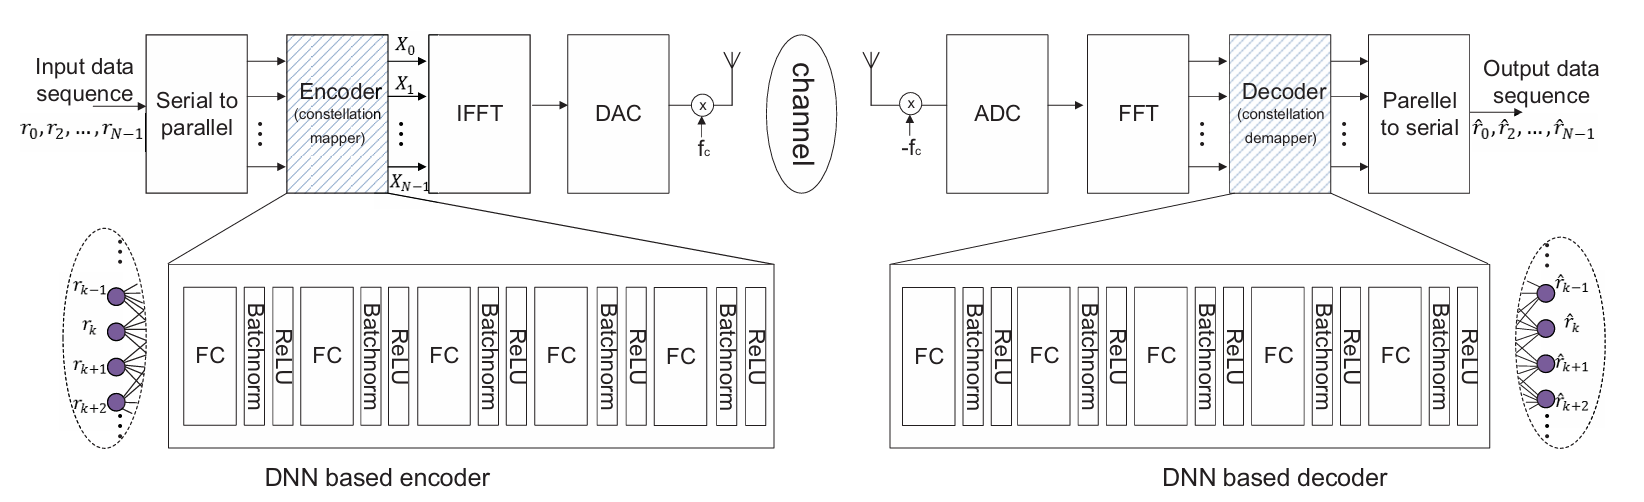
\includegraphics[width=0.85\linewidth]{prnet_architecture.png}
    \end{center}
    Standard modulation and demodulation are completely replaced by a \textbf{DNN encoder and decoder} sharing a symmetric topology: a \textbf{128-node input layer} (I/Q representation) feeding into 5 hidden layers (2048 nodes each) and a \textbf{128-node output layer}. Each hidden sub-block applies \textbf{FC} $\rightarrow$ \textbf{Batch Norm} $\rightarrow$ \textbf{ReLU}:
    \begin{itemize}
        \item \textbf{FC:} Dense connectivity enables joint subcarrier processing.
        \item \textbf{BN:} Stabilises training to prevent gradient collapse.
        \item \textbf{ReLU:} Provides non-linearity for non-convex PAPR--BER mappings.
    \end{itemize}

    \textit{Note: The final output layer is \textbf{strictly linear} (no BN/ReLU) to output unbounded I/Q spatial coordinates (detailed on next slide).}

\end{frame}

% ==========================================================================
% SLIDE 3: SYSTEM MODEL & INPUT REPRESENTATION
% ==========================================================================
\begin{frame}[t]{End-to-End System Model}

    \fontsize{13}{17}\selectfont
    \setlength{\abovedisplayskip}{3pt}
    \setlength{\belowdisplayskip}{3pt}
    \setlength{\parskip}{1pt}
    \vspace*{1.8in}

    \textbf{1. Input Representation:} Real I/Q vector
    \begin{equation*}
        \bm{r} = [I_0,\, Q_0,\, \dots,\, I_{N-1},\, Q_{N-1}]^T \in \mathbb{R}^{2N}
    \end{equation*}

    \textbf{2. DNN Encoder:} $f$ parameterized by weights $\theta_f$
    \begin{equation*}
        \bm{X} = f(\bm{r};\,\theta_f) \in \mathbb{C}^N
    \end{equation*}

    \textbf{3. OFDM Mod \& Channel:} IFFT, then Rayleigh fading $\mathbb{H}$ \& AWGN
    \begin{equation*}
        y[n] = \mathbb{H}\bigl(\mathrm{IFFT}(\bm{X})\bigr)
    \end{equation*}

    \textbf{4. Demod \& EQ:} FFT to frequency domain, zero-forcing
    \begin{equation*}
        \hat{Y}_k = X_k + \frac{E_k}{H_k}
    \end{equation*}

    \textbf{5. DNN Decoder:} $g$ parameterized by weights $\theta_g$
    \begin{equation*}
        \hat{\bm{r}} = g(\hat{\bm{Y}};\,\theta_g) \in \mathbb{R}^{2N}
    \end{equation*}

    \textbf{6. Fully Differentiable End-to-End Chain:}
    \begin{equation*}
        \hat{\bm{r}} = g \circ \mathrm{FFT} \circ \mathbb{H} \circ \mathrm{IFFT} \circ f(\bm{r})
    \end{equation*}

    \vspace{0.15in}
    \setbeamertemplate{blocks}[rounded][shadow=true]
    \setbeamerfont{block title}{size=\fontsize{14}{18}\selectfont,series=\bfseries}
    \setbeamercolor{block title}{bg=blue!80!black,fg=white}
    \setbeamercolor{block body}{bg=blue!10,fg=black}
    \begin{block}{Why I/Q?}
        Unlike categorical one-hot encoding, continuous I/Q decomposition strictly halves the input dimension (128 vs.\ 256), allows the network to optimise continuous spatial coordinate geometry directly, and enables explicit per-symbol power normalisation ($\mathbb{E}[|X|^2] = 1$).
    \end{block}

\end{frame}

% ==========================================================================
% SLIDE 4: JOINT OPTIMIZATION & LOSS FUNCTION
% ==========================================================================
\begin{frame}[t]{Joint Optimization \& Multi-Objective Loss}

    \fontsize{13}{17}\selectfont
    \setlength{\abovedisplayskip}{3pt}
    \setlength{\belowdisplayskip}{3pt}
    \setlength{\parskip}{1pt}
    \vspace*{1.8in}

    \textbf{Reconstruction loss} (MSE in $\mathbb{R}^{2N}$):
    \begin{equation*}
        \mathcal{L}_1(\bm{r},\hat{\bm{r}})
        = \frac{1}{2N}\bigl\|\bm{r} - g\bigl(\mathrm{FFT} \circ \mathbb{H} \circ \mathrm{IFFT}\bigl(f(\bm{r};\,\theta_f)\bigr);\,\theta_g\bigr)\bigr\|_2^2
        = \frac{1}{2N}\sum_{i=0}^{2N-1}\bigl(r_i - \hat{r}_i\bigr)^2
    \end{equation*}

    \textbf{PAPR penalty} (oversampled time-domain waveform, $L \ge 4$):
    \begin{equation*}
        \mathcal{L}_2(\bm{r})
        = \mathrm{PAPR}\bigl\{\mathrm{IFFT}\bigl(f(\bm{r};\,\theta_f)\bigr)\bigr\}
        = \frac{\displaystyle\max_{0 \le n \le NL-1} |x[n]|^2}
        {\displaystyle\frac{1}{NL}\sum_{n=0}^{NL-1}|x[n]|^2}
    \end{equation*}

    \textbf{Joint loss:} ($\lambda$ governs the BER--PAPR trade-off)
    \begin{equation*}
        \mathcal{L}(\bm{r},\hat{\bm{r}}) = \mathcal{L}_1(\bm{r},\hat{\bm{r}}) + \lambda\,\mathcal{L}_2(\bm{r})
    \end{equation*}

    \vspace{0.15in}
    \setbeamertemplate{blocks}[rounded][shadow=true]
    \setbeamerfont{block title}{size=\fontsize{14}{18}\selectfont,series=\bfseries}
    \setbeamercolor{block title}{bg=blue!80!black,fg=white}
    \setbeamercolor{block body}{bg=blue!10,fg=black}
    \begin{block}{Why Regression MSE?}
        The original PRNet formulation uses \textbf{Cross-Entropy loss} for categorical, one-hot encoded inputs. Because our system adopts a \textbf{continuous I/Q parameterization}, the reconstruction task becomes a regression problem. Therefore, we utilize \textbf{Mean Squared Error (MSE)} to compute the loss in the $2N$-dimensional real-valued signal space.
    \end{block}

\end{frame}

% ==========================================================================
% SLIDE 5: TWO-STAGE TRAINING METHODOLOGY
% ==========================================================================
\begin{frame}[t]{Two-Stage Training Methodology}

    \fontsize{12}{15}\selectfont
    \setlength{\abovedisplayskip}{3pt}
    \setlength{\belowdisplayskip}{3pt}
    \setlength{\parskip}{1pt}
    \vspace*{1.8in}

    \textbf{Denoising autoencoder:} Artificial noise at a corruption level $\eta$ (noise-to-signal ratio) is injected during the forward pass to simulate the physical channel and force the decoder to learn robust decision boundaries.

    \begin{columns}[T,onlytextwidth]
        \begin{column}{0.48\textwidth}
            \textbf{Stage~1 --- Noise Selection} ($\lambda = 0$):
            Sweep $\eta$ while training with reconstruction loss $\mathcal{L}_1$ only.

            \begin{center}
                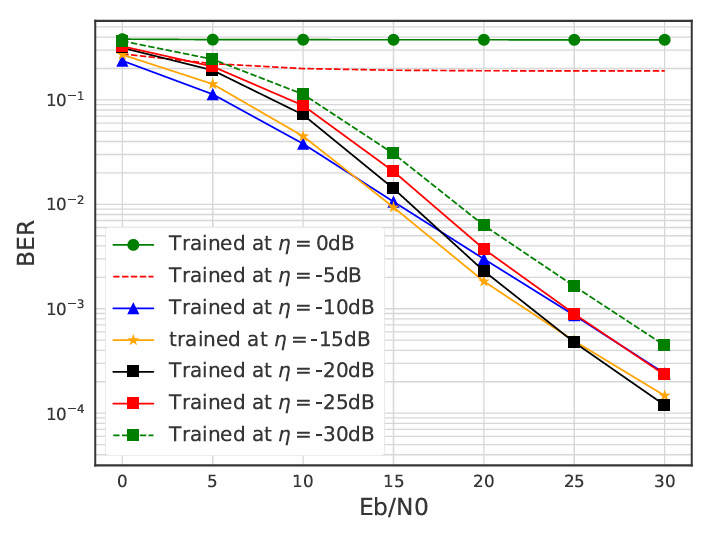
\includegraphics[width=0.8\linewidth]{prnet_ber_corruption.png}
            \end{center}

            For excessive corruption levels ($\eta = 0$ and $-5$~dB), the model fails to learn meaningful boundaries entirely, while at very low corruption levels ($\eta = -30$~dB) it overfits to the noiseless scenario. The best point is $\eta^\star = -15$~dB; any divergence from this optimal point steadily increases the overall BER.
        \end{column}

        \begin{column}{0.48\textwidth}
            \textbf{Stage~2 --- Trade-Off Training} ($\eta = \eta^\star$):
            Sweep penalty weight $\lambda$ under the full loss $\mathcal{L} = \mathcal{L}_1 + \lambda\,\mathcal{L}_2$.

            \begin{center}
                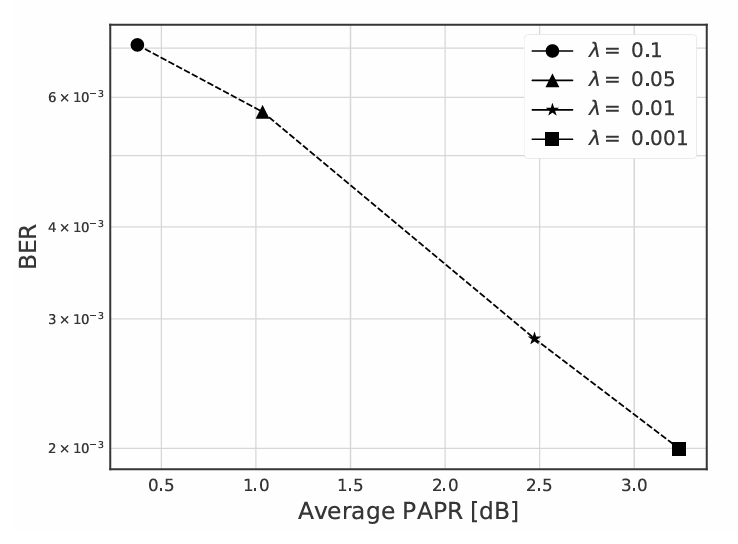
\includegraphics[width=0.8\linewidth]{prnet_ber_papr_lambda.png}
            \end{center}

            As $\lambda$ increases, PAPR decreases monotonically while the BER increases. Heavy penalties ($\lambda = 0.1$) aggressively squash the waveform but severely compromise the error rate, whereas minimal penalties ($\lambda = 0.001$) prioritize low BER at the expense of higher PAPR. The ideal operating point is $\lambda = 0.01$, achieving meaningful PAPR reduction without severely degrading the BER baseline.
        \end{column}
    \end{columns}

\end{frame}

% ==========================================================================
% SLIDE 6: LEARNED CONSTELLATION SHAPING
% ==========================================================================
\begin{frame}{Learned Constellation Shaping}

    \fontsize{12}{15}\selectfont
    \vspace*{1in}

    \begin{center}
        
\includegraphics[width=0.35\linewidth]{encoder_constellation_rayleigh.jpg}
    \end{center}

    \vspace{0.1in}
    Unlike classical OFDM with rigid QPSK boundaries, the PRNet encoder \textbf{dynamically disperses} constellation points:

    \begin{itemize}
        \item Maps discrete input data into a \textbf{continuous, cloud-like} spatial distribution.
        \item Trades traditional Euclidean spacing for optimal PAPR reduction.
        \item The jointly trained decoder learns to recover data from this custom distribution without explicit knowledge of the mapping.
    \end{itemize}

\end{frame}

% ==========================================================================
% SLIDE 7: BER PERFORMANCE (AUTHOR vs. REPRODUCED)
% ==========================================================================
\begin{frame}{BER Performance: Validation}

    \fontsize{12}{15}\selectfont

    \begin{columns}[T]
        \begin{column}{0.48\textwidth}
            \begin{center}
                \textbf{Original Paper}
                \vspace{0.1cm}

                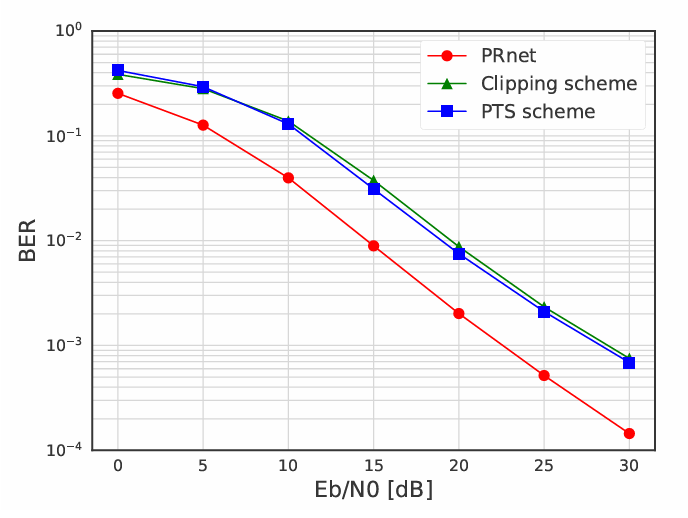
\includegraphics[width=0.95\linewidth]{prnet_ber.png}
            \end{center}
        \end{column}
        \begin{column}{0.48\textwidth}
            \begin{center}
                \textbf{Our Reproduction}
                \vspace{0.1cm}

                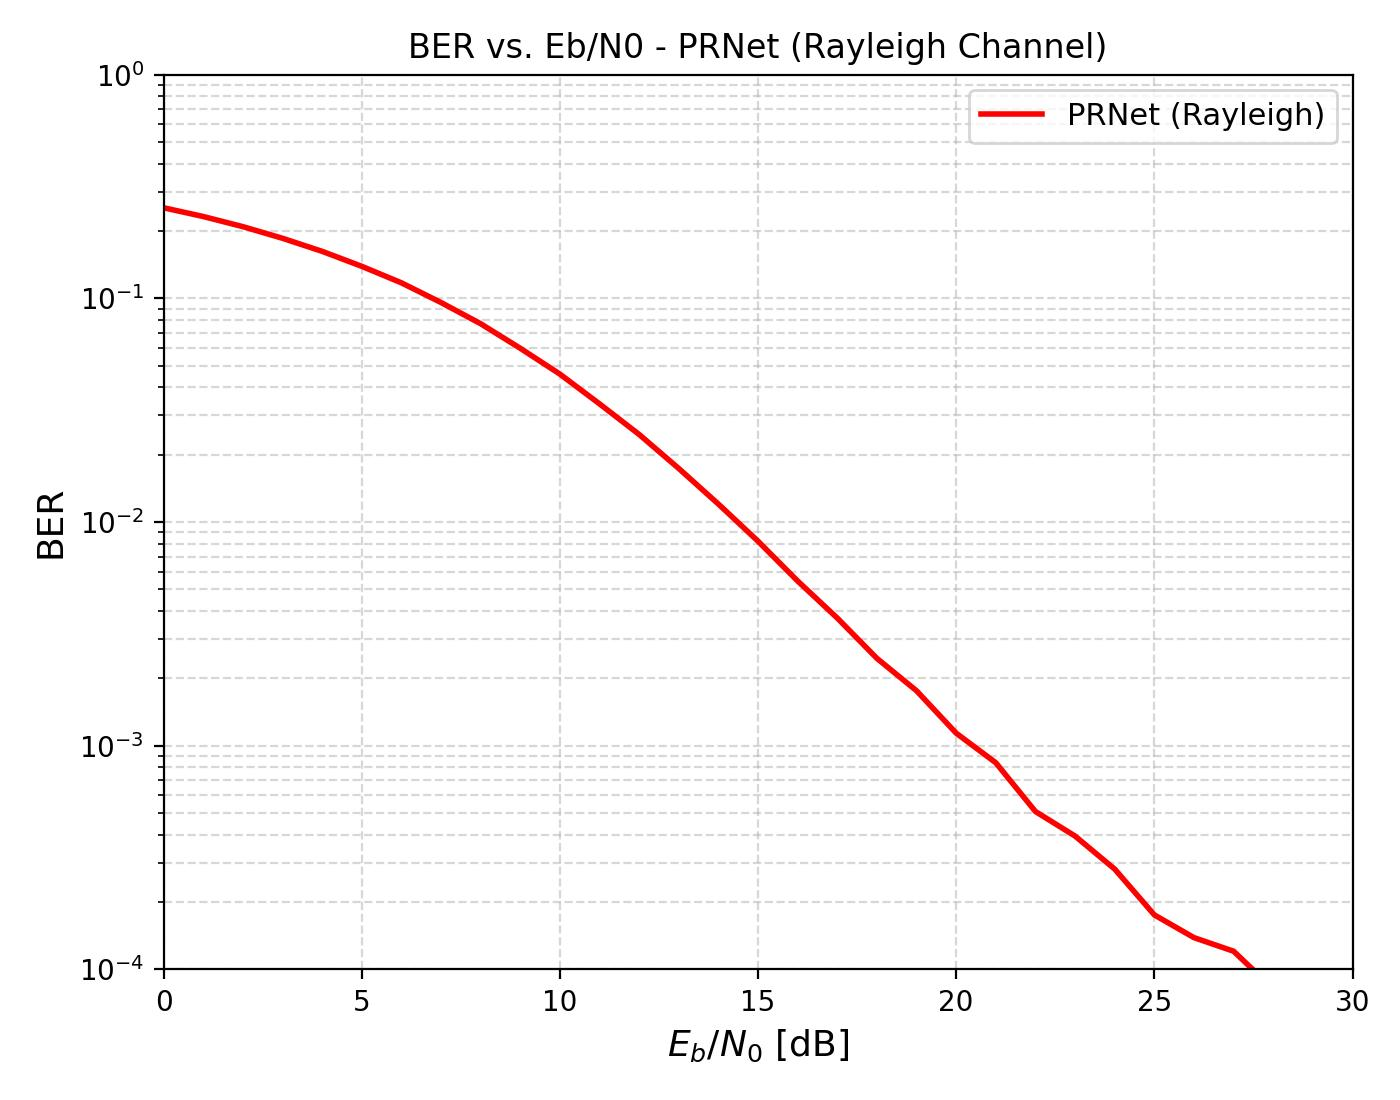
\includegraphics[width=0.95\linewidth]{ber_vs_snr_rayleigh.jpg}
            \end{center}
        \end{column}
    \end{columns}

    \vspace{0.2cm}
    \begin{itemize}
        \item PRNet \textbf{outperforms} the theoretical QPSK baseline --- learns
              an implicit coding gain under the Rayleigh fading channel.
        \item Deterministic inference: single forward pass, no side information required.
    \end{itemize}

\end{frame}

% ==========================================================================
% SLIDE 7: PAPR REDUCTION (AUTHOR vs. REPRODUCED)
% ==========================================================================
\begin{frame}{PAPR Reduction \& Proxy Metric Discrepancy}

    \fontsize{11}{14}\selectfont

    \begin{columns}[T]
        \begin{column}{0.48\textwidth}
            \begin{center}
                \textbf{Original Paper}
                \vspace{0.05cm}

                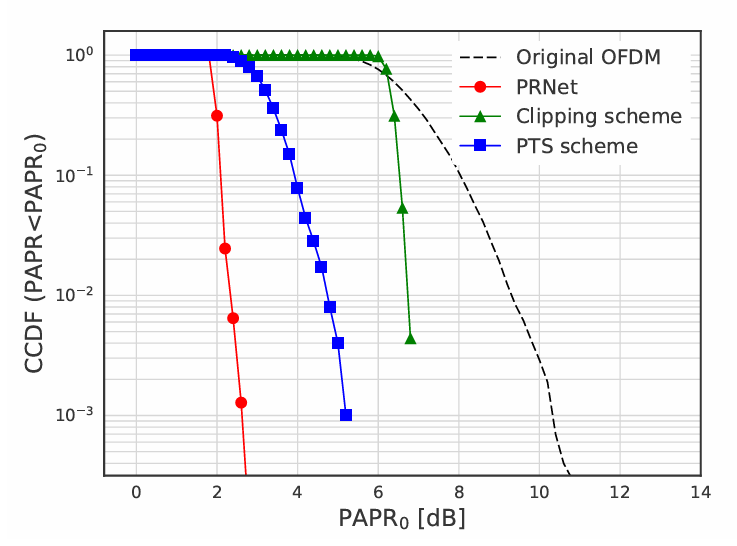
\includegraphics[width=0.85\linewidth]{prnet_ccdf.png}
            \end{center}
        \end{column}
        \begin{column}{0.48\textwidth}
            \begin{center}
                \textbf{Our Reproduction}
                \vspace{0.05cm}

                
\includegraphics[width=0.85\linewidth]{ccdf_papr_rayleigh.jpg}
            \end{center}
        \end{column}
    \end{columns}

    \vspace{0.1cm}
    \textbf{Metric Mismatch:} The authors used an amplitude-based proxy instead of physical power:
    \begin{itemize}
        \item \textbf{Authors' proxy:} $\mathrm{PAPR}_{\mathrm{proxy}}\,\mathrm{[dB]} = 10\log_{10}\!\bigl(\max_n |x_{\mathrm{norm}}[n]|\bigr) \Rightarrow \text{Reports } 3\text{ dB}$
        \item \textbf{Standard metric:} $\mathrm{PAPR}_{\mathrm{std}}\,\mathrm{[dB]} = 10\log_{10}\!\bigl(\max_n |x_{\mathrm{norm}}[n]|^2\bigr) = 2 \times \mathrm{PAPR}_{\mathrm{proxy}}\,\mathrm{[dB]} \Rightarrow \text{Actually } 6\text{ dB}$
    \end{itemize}

    \vspace{0.1cm}
    Despite this $2\times$ discrepancy, PRNet still achieves a \textbf{substantial $4$--$5$~dB reduction} vs.\ original OFDM ($\approx 10.5$~dB).

\end{frame}


% ==========================================================================
% SLIDE 8: COMPUTATIONAL COMPLEXITY & LIMITATIONS
% ==========================================================================
\begin{frame}{Computational Complexity \& Limitations}

    \fontsize{13}{17}\selectfont
    \textbf{Complexity Correction:}
    \begin{itemize}
        \item Original claim: $\mathcal{O}(L \cdot K \cdot M)$.
        \item \textbf{True complexity:} $\mathcal{O}(L \cdot K^2)$ --- hidden-layer
              matrix multiplications ($K = 2048$) dominate; independent of $M$.
        \item GPU inference: $480\;\mu\text{s}$ vs.\ PTS: $2{,}890\;\mu\text{s}$
              ($\approx 6\times$ speedup).
    \end{itemize}

    \vspace{0.3cm}
    \textbf{Practical Limitations of PRNet:}
    \begin{itemize}
        \item \textbf{Scalability:} FC layers scale as $\mathcal{O}(N^2)$ ---
              impractical for commercial $N = 1024$.
        \item \textbf{Channel mismatch:} Overfits to the training fading model;
              degrades under unmodelled conditions.
        \item \textbf{Configuration rigidity:} Changing $N$ or $M$ requires full
              architectural redesign and retraining.
        \item \textbf{Interpretability:} Black-box weights prevent worst-case
              guarantees required by telecom standards.
    \end{itemize}

\end{frame}

\end{document}